%==========================================================================
%Template File for Evolutionary Computation Symposium
%==========================================================================
\documentclass[a4paper,11pt,twocolumn]{jarticle}
\usepackage{evocomp}
\usepackage{fancyhdr}
\usepackage[linesnumbered,ruled]{algorithm2e}
\usepackage{graphicx}
\usepackage{subcaption}

\pagestyle{empty}

\renewcommand{\headrulewidth}{0.0pt}
\renewcommand{\footrulewidth}{0.0pt}

\renewcommand\refname{References}

\begin{document}
\twocolumn[%
\begin{center}

\beginheader

\jtitle%
{Cyclic Simple Evolutionary Algorithm and Bit Climber for Constrained Multi-Objective Optimization}

\begin{authors}
\name{1}{Felipe Honjo Ide},
\name{1}{Hernan Aguirre},
\name{1}{Kiyoshi Tanaka},
\end{authors}



\begin{affiliation}
\aff{1}{Graduate School of Medicine, Science and Technology, Shinshu University},
\end{affiliation}

\endheader

\end{center}
]

\etitle{Cyclic Simple Evolutionary Algorithm and Bit Climber for Constrained Multi-Objective Optimization}

\ename{1}{Felipe Honjo Ide(22hs204k@shinshu-u.ac.jp)}
\ename{1}{Hernan Aguirre(ahernan@shinshu-u.ac.jp)}
\ename{1}{Kiyoshi Tanaka(ktanaka@shinshu-u.ac.jp)}

\eaff{1}{%
Graduate School of Medicine, Science and Technology, Shinshu University
}

\vspace{3mm}

\kanjiskip=.1zw plus 3pt minus 3pt
\xkanjiskip=.1zw plus 3pt minus 3pt

\section{Introduction}

Many real-world optimization problems require the simultaneous optimization of more than one objective, where the improvement in one objective is often accompanied by the detriment in other objectives. These problems are known as Multi-Objective Optimization Problems (MOPs). In addition, MOPs also often contain one or more constraints. These Constrained Multi-Objective Optimization Problems (CMOPs) have a portion of solutions that are infeasible.

To solve these MOPs, Multi-Objective Evolutionary Algorithms (MOEAs) have been constantly developed and improved on. MOEAs use the concepts of natural evolution, such as selection, reproduction and mutation to iterate over candidate solutions over a given number of generations, until a set of satisfactory solutions have been found. In order to handle infeasible solutions of CMOPs, Constraint Handling Techniques (CHTs) have been added to existing MOEAs, and even Constrained Multi-Evolutionary Algorithms (CMOEAs), which are built from the ground up to deal with infeasible solutions, have been proposed over the years.

Although a lot of work has been done in the continuous domain, only a few CMOEAs focus in binary problems, and even fewer are dedicated to solving highly constrained problems.

From this standpoint, in this work, we focus on binary CMOPs, and propose a new CMOEA that cycles between a $(\mu + \lambda)$ Simple Evolutionary Algorithm (SEA) and a Multi-Objective Random Bit-Climber (moRBC) \cite{Aguirre_2005}, named C-EA-RBC. The SEA optimizes the constraint violation of infeasible solutions with the goal of finding feasible solutions, and the moRBC climbs feasible solutions aiming to find additional non-dominated feasible solutions. In this work, we detail how C-EA-RBC works, compare its performance to other state-of-the-art CMOEAs when solving SAT Constrained MNK-Landscapes, and analyze its properties in regards to optimizing the constraint violations and finding feasible solutions.

The remainder of this work is organized as follows. Section 2 presents the relevant concepts of CMOPs and CMOEAs. Section 3 details the proposed MOEA, C-EA-RBC. Then, Section 4 explains the experimental setup, and Section 5 presents the experimental results and discussions. Lastly, Section 5 concludes this work and reflects on possible future works.

\section{Constrained Multi-Objective Evolutionary Algorithms}

Constrained binary multi-objective problems can be mathematically represented as:

\vskip-15pt
\begin{equation} \label{eq:MOP}
	\begin{aligned}
		\text{maximize} & ~~\mathbf{f} = (f_1(\mathbf{x}), f_2(\mathbf{x}), \dots, f_M(\mathbf{x})) \\ 
		\text{subject to} & ~~\mathbf{x} =(x_1, x_2, \dots, x_N), \:x_i \in \{0,1\} \\
		& ~~h^o_j(\mathbf{x}) = 0, ~~j = 1,\dots,p^o \\
		& ~~g^o_k(\mathbf{x}) \leq 0, ~~k = 1,\dots,q^o \text{,}
	\end{aligned}
\end{equation}
%\vspace{-0.4cm}

\noindent where $M$ functions $f_i$ need to be simultaneously optimized, while satisfying all $p^o$ equality and $q^o$ inequality constraints defined by the functions $h^o_k(\mathbf{x})$ and $g^o_j(\mathbf{x})$, respectively. 

Given two solutions $\mathbf{x}_a$ and $\mathbf{x}_b$, $\mathbf{x}_a$ is said to dominate $\mathbf{x}_b$, or $\mathbf{f}(\mathbf{x}_a) \succ \mathbf{f}(\mathbf{x}_b)$, if and only if $\forall i$ $f_i(\mathbf{x}_a) \geq f_i(\mathbf{x}_b)$ and $\exists i$ $f_i(\mathbf{x}_a) > f_i(\mathbf{x}_b)$, $i=1,2,\dots,M$. On the other hand, $\mathbf{x}_a$ and $\mathbf{x}_b$ are said to be non-dominated by each other if neither $\mathbf{f}(\mathbf{x}_a) \succ \mathbf{f}(\mathbf{x}_b)$ nor $\mathbf{f}(\mathbf{x}_b) \succ \mathbf{f}(\mathbf{x}_a)$. The objective vectors of the set of non-dominated solutions of a given problem is called the Pareto Front (PF).

If a solutions satisfies the constraints, it is called a feasible solution, and can be considered a valid solution for the CMOP. Otherwise, it is called an infeasible solution, and its constraint violation value can be used to compute its distance to feasibility, which represents how far this solution is from being considered feasible.

To solve these CMOPs, many Constraint Handling Techniques (CHTs) and Constrained Multi-Objective Evolutionary Algorithms (CMOEAs) have been proposed over the years. Some of the most well known ones are constraints dominance, in which feasible solutions are ranked over infeasible ones, but the latter are allowed to survive to the next generation, given that it does not exceed the population size limit \cite{Deb_2002}, penalty functions, in which the fitness function of the infeasible solutions are penalized according to their distance to feasibility \cite{Smith_1997} and co-evolutionary strategies, in which the solver evolves two populations separately that have different optimization goals \cite{Coello_2000}.

%To solve these CMOPs, many Constraint Handling Techniques (CHTs) and Constrained Multi-Objective Evolutionary Algorithms (CMOEAs) have been proposed over the years. The strategy that they use to handle infeasible solutions can be generally divided into four types \cite{Bao_2022}. In the first one, the objective functions are prioritized over the constraint violation, such as in Death Penalty, in which all infeasible solutions are eliminated \cite{Mezura_2011} and Constraints Dominance, in which feasible solutions are ranked over infeasible ones, but the latter are allowed to survive to the next generation, given that it does not exceed the population size limit \cite{Deb_2002, Muhammad_2013}.
%
%The second type of CMOPs make use of the information gained from infeasible solutions, such as in penalty functions, in which the fitness function of the infeasible solutions are penalized according to their distance to feasibility \cite{Smith_1997, Woldesenbet_2009, Jeffrey_1994, Takahima_2005}, in IDEA, that counts the constraints violation as an addition objective \cite{Ray_2009}, and in MOEA/D-ACDP, in which the dominance relationship depends on the angle between solutions and the ratio of feasible solutions in the population \cite{Zhun_2019}.
%
%In the third type, Co-Evolutionary strategies \cite{Coello_2000} are used, such as using separate populations to optimize convergence and diversity separately, in C-TAEA \cite{Li_2019}, and using separate populations to optimize only the objective functions in one population, and to optimize the whole problem in another, in CCMO \cite{Tian_2020}.
%
%In addition, many other miscellaneous strategies were developed such as ToP, which transforms the problem into a constrained single-objective problem \cite{Liu_2019} and MOEA/D-PPS, which divides the search into one stage that optimizes the objective functions only, and the second stage that repairs the infeasible solutions found \cite{Fan_2019}.

\section{Proposed algorithm}

Here, we propose an MOEA for constrained binary benchmark problems that alternates between a simple evolutionary algorithm (SEA), that optimizes constraint violation, and a multi-objective Random Bit Climber (moRBC), that optimizes the objective functions. In this section, we describe the general framework of the proposed algorithm, then detail both SEA and moRBC, and how the contribution between the two are done.

\subsection{General Framework}

%The proposed algorithm, name Cyclic Evolutionary Algorithm and Random Bit Climber (C-EA-RBC) works by either optimizing the violation values of infeasible solutions by a simple evolutionary algorithm until at least one feasible solution has been found, or by optimizing the objective functions of feasible solutions until all feasible solutions have been exhausted. 

Algorithm \ref{alg:cearbc} shows the general framework of C-EA-RBC. More details of SEA and morBC are given in the following subsections.

%The general framework of C-EA-RBC is shown in the flowchart of Fig. \ref{fig:CEARBC}, and Algorithm \ref{alg:cearbc}. More details of SEA and morBC are given in the following subsections. The flow of C-EA-RBC is described as follows.

%\begin{figure}[b!]
%	\centering
%	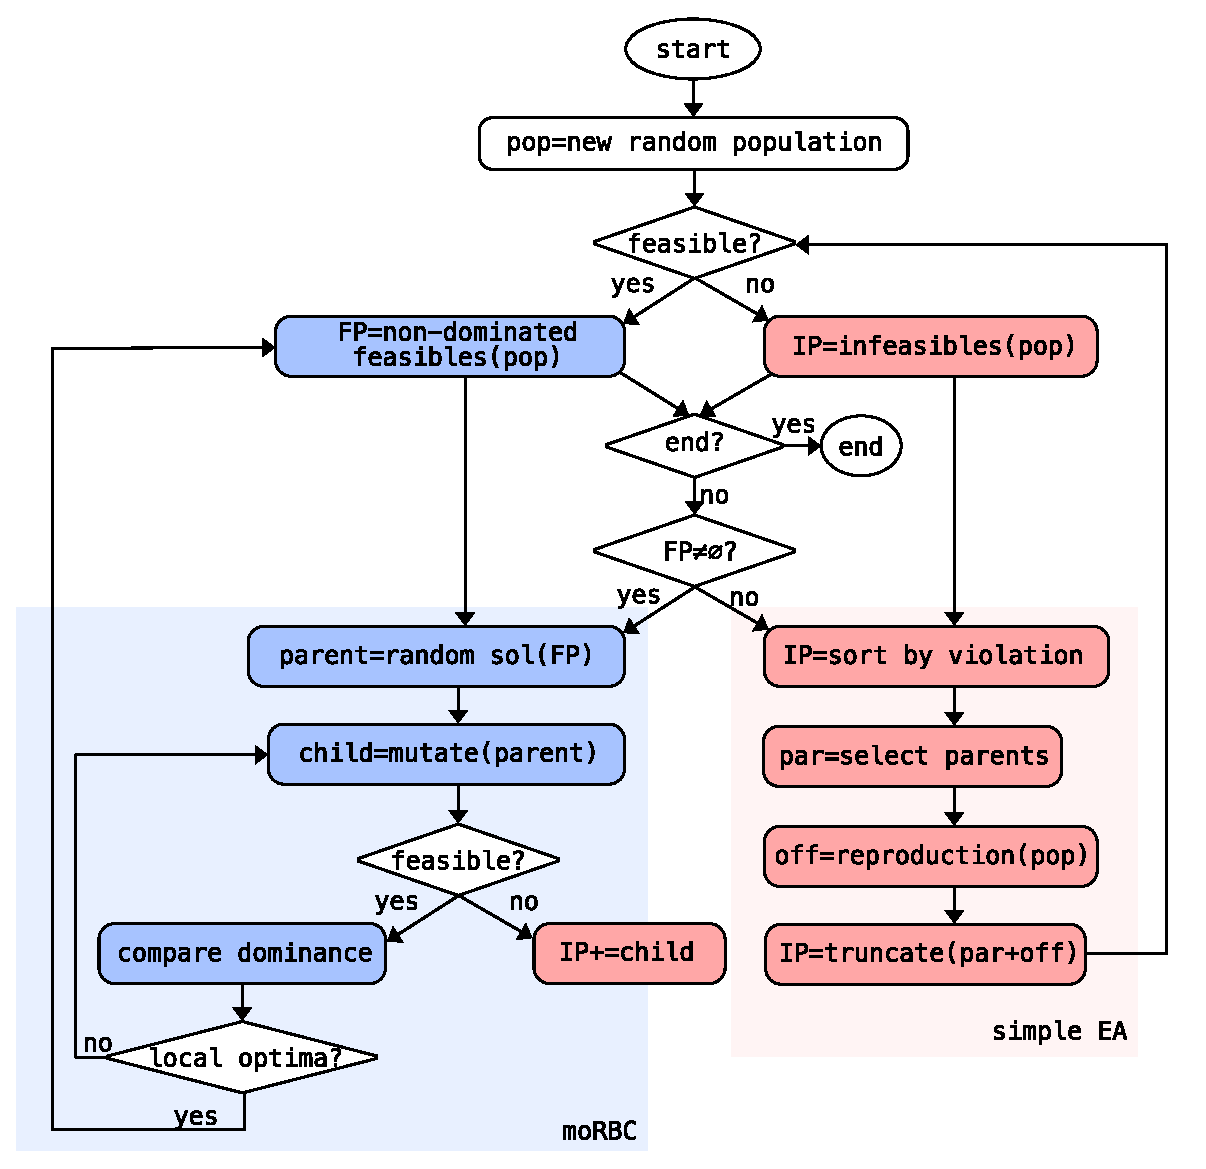
\includegraphics[width=\columnwidth]{figs/CEARBC.eps}
%	\caption{Flowchart of C-EA-RBC.}
%	\label{fig:CEARBC}
%\end{figure}

C-EA-RBC starts by initializing a random population, which is divided into two populations of feasible solutions $FP$, and infeasible solutions $IP$. If at least one feasible solution is found, it executes the moRBC until all feasible solutions are exhausted. When no feasible solutions are available, it executes the SEA until at least one feasible solutions is found, and the algorithm switches to moRBC. This is repeated until the number of fitness evaluations have been exhausted. C-EA-RBC can switch between its two stages multiple times in one execution.

\begin{algorithm}[t!]
	\caption{Framework of C-EA-RBC.}
	\label{alg:cearbc}
	\KwData{$N$}
	$P \gets$ New random initial population\;
	$P \gets evaluate(P)$\;
	$IP \gets infeasibles(P)$\;
	$FP \gets feasibles(P)$\; 
	\While {\textit{termination criteria not fulfilled}} {
		\uIf{$FP = \emptyset$} {
			$FP, IP \gets SEA()$;  \tcp{Alg. \ref{alg:sea}}
		}
		\uElse {
			$FP, IP \gets moRBC()$;  \tcp{Alg. \ref{alg:RBC}}
		}
	}
	\Return $archive$\;
\end{algorithm}

\begin{algorithm}[t!]
	\caption{SEA used in C-EA-RBC.}
	\label{alg:sea}
	\KwData{$IP$, $FP$}
	$FP \gets$ $violation\_sorting(FP)$\;
	\While {\textit{termination criteria not fulfilled}} {
		$parents \gets selection(FP$)\;
		$offsprints \gets reproduction(parents)$\;
		$offsprints \gets evaluate(offsprings)$\;
		$FP \gets feasibles(offsprings)$\;
		$IP = survival\_selection(parents+offsprings)$\;
		\uIf{$FP \neq \emptyset$} {
			\Return $FP, IP$;
		}
	}
	\Return $FP, IP$\;
\end{algorithm}

\begin{algorithm}[t!]
	\caption{moRBC used in C-EA-RBC.}
	\label{alg:RBC}
	\KwData{$N$, $IP$, $FP$}
	$i \gets 0$\;
	$steps \gets 0$\;
	$parent$ $\gets$ $random\_solution(FP)$\;
	$PO \gets$ New random permutation order\;
	\While {\textit{termination criteria not fulfilled}} {
		$child \gets$ \textit{mutate}($parent$, \textit{PO}[\textit{i}])\;
		$steps++$\;
		\uIf{$feasibility(child) = false$} {
			$IP \gets UpdateIP(child)$\;
		}
		\uElse {
			\uIf{$child \succ parent$} {
				delete parent\;
				$parent$ $\gets$ $child$\;
				$steps \gets 0$\;
			}
			\uElseIf {$parent \succ child$} {
				delete child\;
			}
			\uElse {
				$FP \gets UpdateFP(child)$\;
			}
		}
		$i \gets (i+1)\%N$\;
		\uIf{$steps=N$} {
			$FP \gets UpdateFP(parent)$\;
			\uIf{$FP \neq \emptyset$} {
				$parent \gets restart(FP)$\;
				$i \gets 0$\;
				$steps \gets 0$\;
				$PO \gets$ New random permutation order\;
			}
			\uElse{
				\Return $FP, IP$\;
			}
		}
	}
	\Return $FP, IP$\;
\end{algorithm}

\subsection{Simple Evolutionary Algorithm}

SEA is a single objective optimizer that aims to minimize the constraint violation of the solutions in $IP$ until at least one feasible solution is found. Algorithm \ref{alg:sea} describes the SEA used in this work.

SEA is a population-based algorithm that uses binary tournament to select parents for crossover, then creates offspring solutions using binary crossover and bit-flip mutation, and the surviving solutions are ranked by the sum of the constraint violations of all constraints of the problem. The number of solutions in $IP$ is kept at a maximum size by truncation.

When feasible solutions are found, they are added to $FP$, SEA stops its execution and C-EA-RBC switches to moRBC.

\subsection{Multi-Objective Random Bit Climber}

moRBC is a hill climbing algorithm that has been studied thoroughly over the years, and many extensions have been proposed. In this work we extend moRBC to handle infeasible solutions found during its run. Its pseudo-algorithm is given in Algorithm \ref{alg:RBC} and described as follows.

moRBC starts with a randomly chosen solution from $FP$ and creates a child by doing one-bit-flip mutation. If the child is infeasible, it is added to $IP$, ensuring that $IP$ is ordered by constraint violation and kept at its size limit. If the child if feasible, then a dominance comparison is done as follows. If the parent dominates the child, then the child is discarded and the search continues with the parent. If the child dominates the parent, then the child replaces the parent and the search continues with the new parent. If they are non-dominated, then the child is added to $FP$, and the search continues with the parent. This process continues until a local optima has been found, which is added to $FP$. If $FP$ contains at least one non-dominated not-climbed solution, moRBC is restarted with one of those solutions, chosen randomly. Otherwise, it stops execution and switches to SEA. 

\section{Experimental Setup}

In this section, we describe the experimental setup, including the benchmark problem, the MOEAs and the metrics used for analysis.

\subsection{SAT Constrained MNK-Landscapes}

To evaluate the performance of C-EA-RBC, we solve SAT Constrained MNK-Landscapes (SAT-MNK).

MNK-Landscapes are highly configurable binary benchmark problems with tunable number of objectives, variables and epistasis through their parameters $M$, $N$ and $K$, respectively \cite{Aguirre_2004}. They can be mathematically represented as:

%are the extension of well-known mathematical models, NK-Landscapes \cite{Kauffman_1993}, to the multi-objective domain. They 

\vskip-15pt
\begin{equation}
	f_i(\mathbf{x}) = \frac{1}{N}\sum_{j=1}^{N}f_{i,j}(x_j,\underbrace{z_1^{(i,j)},z_2^{(i,j)},\cdots, z_{K_i}^{(i,j)}}_{\text{$K_i$ bits interacting with $x_j$}}),
\end{equation}

\noindent where $f_{i,j}: B^{K_i+1}\rightarrow \mathbb{R}$ gives the fitness contribution of bit $x_j$ to $f_i$, and $z_1^{(i,j)},\dots, z_{K_i}^{(i,j)}$ are the $K_i$ bits interacting with bit $x_j$ in the string $\mathbf{x}$. This means that the fitness value of the bit $x_j$ depends not only on its own value, but also on the other $K_i$ bits that it interacts with \cite{Aguirre_2004, Pelikan_2010}. 
%In depth analysis of the properties of MNK-Landscapes can be found in \cite{Aguirre_2004} and \cite{Hernan_2007}.

Since MNK-Landscapes are unconstrained problems, we attached constraints to them with SAT Constraints. They are highly configurable constraints that can be attached to any benchmark problem. Here we focus only on equality constraints, which are mathematically represented as:

\vskip-20pt
\begin{equation}
	h_j = \sum_{i=1}^{\phi_j}w_{j,i} e(C_{j,i}) = 0 \hspace{1cm}j=1,\dots,p ,
\end{equation} 

%\begin{equation} \label{eq:WSC}
%	g_k = \sum _{i=1}^{\psi_k}w_{k,i} e(C_{k,i}) \le \tau_k \hspace{1cm} k=1,\dots,q,
%\end{equation}

\noindent where:

\vskip-10pt
\begin{equation}
	e(C)=\begin{cases}
		0  \quad \textrm{if } C~\textrm{is true,}\\
		1                \quad \textrm{otherwise.}
	\end{cases}
\end{equation}

%\begin{equation}
%	\tau_k = r \times \sum_{i=1}^{\psi_k}w_{k,i} \hspace{1cm} k=1,\dots,q.
%\end{equation}

%SAT Constraints can have $p$ equality constraints $h$ and $q$ inequality constraints $g$. 

The number of SAT clauses in the SAT Constraints is given by $N_c = \sum_{j=1}^{p}{\phi_j}$. A higher $\phi_j$ value results in a more constrained problem. In this work, we control the difficulty of the problems by the ratio of clauses to variables $\gamma$, which is known to be a common method to adjust the difficulty of SAT Problems \cite{Selman_1996, Nudelman_2004}:

\vskip-10pt
\begin{equation}
	\label{eq:gamma}
	\gamma = \frac{N_c}{N}
\end{equation}

Lastly, the constraint violation is measured by the sum of $w_{j,i}$ of the unsatisfied clauses.

%The total number of clauses in the SAT Constraints is given by $N_c = \sum_{j=1}^{p}{\phi_j} + \sum_{k=1}^{q}{\psi_k}$. We can control the difficulty of the problem by adjusting $\phi_j$ in equality constraints, and $\psi_k$ and $r$ in inequality constraints. 

An important characteristic of SAT-MNK is that PF recedes as $\gamma$ increases, as illustrated in Fig. \ref{fig:sat}. This means that a solver needs to be able to approach the feasible Pareto Front, without getting lost in the infeasible space, where the unconstrained Pareto Front is located.

\begin{figure}[t!]
	\centering
	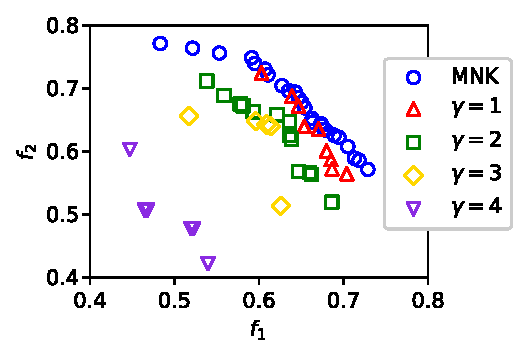
\includegraphics[width=0.7\linewidth]{figs/sat.eps}
	\vskip-5pt
	\caption{PF of SAT-MNK with different $\gamma$.}
	\label{fig:sat}
\end{figure}

We solve MNK-Landscapes with $N=100$, $M=\{2,3,4,5\}$ and $K=\{1,3,5,7\}$, and SAT Constraints with $p=1$, $q=0$ and $\gamma=\{1,2,3,4\}$.

We generate a fixed MNK-Landscape instance and randomly generate 30 SAT Constraint instances for each problem configuration. With that, overall, we use 300 problem instances in this study.

\subsection{Compared MOEAs}

We compare C-EA-RBC with 5 other state-of-the-art MOEAs, namely NSGA-II, CCMO, IDEA, MOEA/D-ACDP and PPS-MOEA/D. The parameters of all MOEAs are the same as the ones proposed in their original papers. 

All MOEAs use population size of $100$ individuals, one-point crossover with probability $1.0$ and bit-flip mutation with probability $1/N$. IDEA uses $\alpha=0.2$, MOEA/D based solvers use the Tchebycheff decomposition method, neighborhood size of 10 individuals, probability of selecting neighboring individuals of $0.9$ and maximum number of replaced individuals of 2. MOEA/D-ACDP uses $\alpha=0.9$ and $\theta(0)=\frac{\pi}{2|P|}$ and PPS-MOEA/D uses $T_c=400$, $\alpha=0.95$, $\tau=0.1$, $cp=2$ and $l=10$.

We evaluate the performance of the MOEAs by the Hypervolume (HV) metric \cite{Zitzler_1999} with reference point at $[0.0,...,0.0]$, and calculate the average HV for the 30 SAT instances over 500 generations. Plot points in which the HV is 0.0 due to the population being composed of only infeasible solutions are not counted towards this metric.

\begin{figure*}[t!]
	\begin{subfigure}{\columnwidth}
		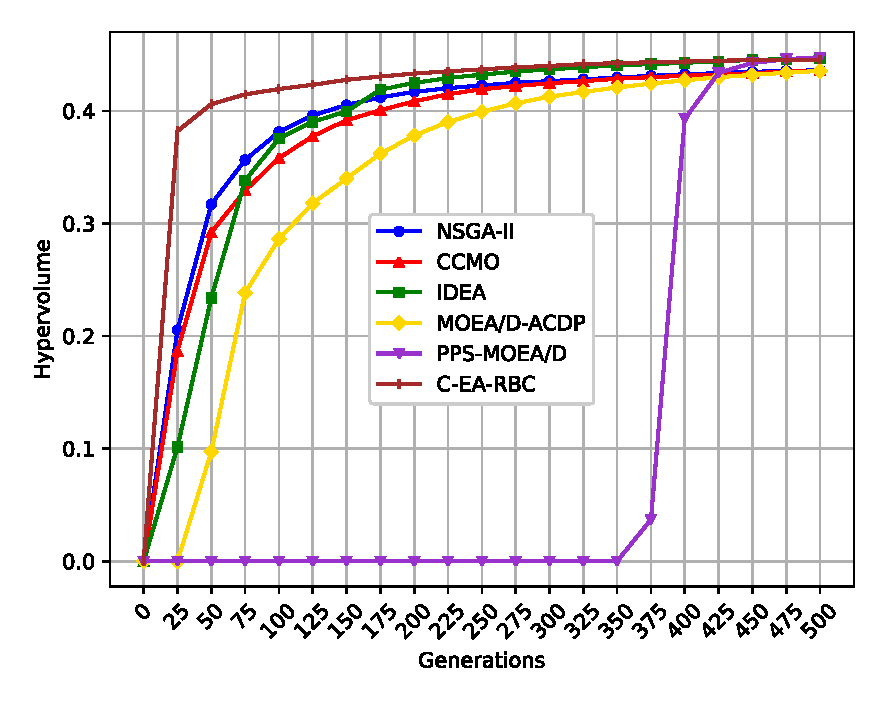
\includegraphics[width=\columnwidth]{figs/HV_gamma100.eps}
		\vskip-5pt
		\caption{$\gamma=1$.}
		\label{fig:HV_gamma100}
	\end{subfigure}\hfill
	\begin{subfigure}{\columnwidth}
		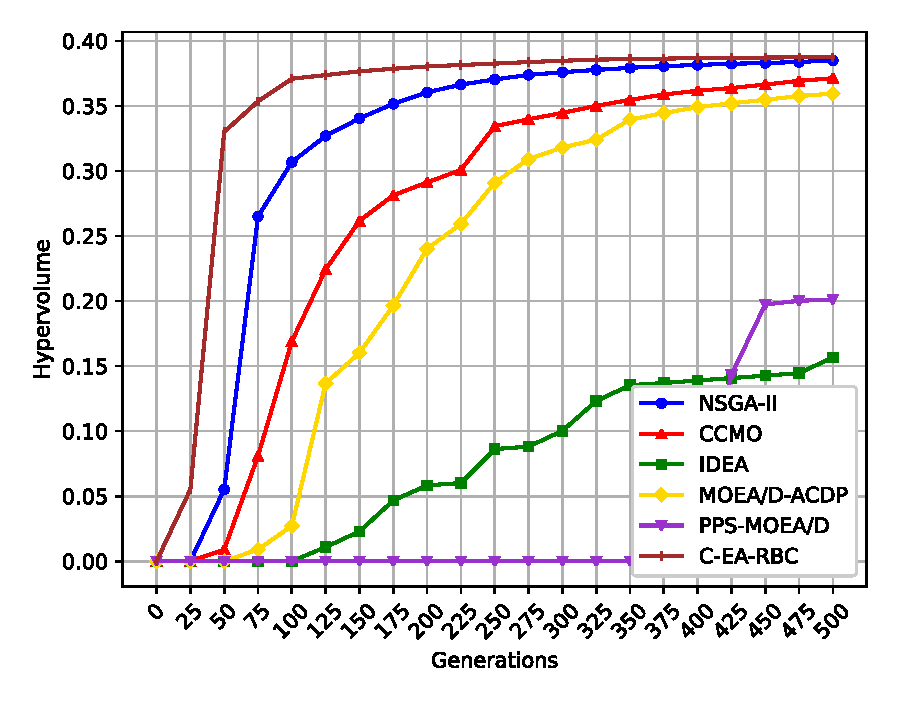
\includegraphics[width=\columnwidth]{figs/HV_gamma200.eps}
		\vskip-5pt
		\caption{$\gamma=2$}
		\label{fig:HV_gamma200}
		
	\end{subfigure}\hfill
	\begin{subfigure}{\columnwidth}
		\includegraphics[width=\columnwidth]{figs/HV_gamma300.eps}
		\vskip-5pt
		\caption{$\gamma=3$.}
		\label{fig:HV_gamma300}
	\end{subfigure}\hfill
	\begin{subfigure}{\columnwidth}
		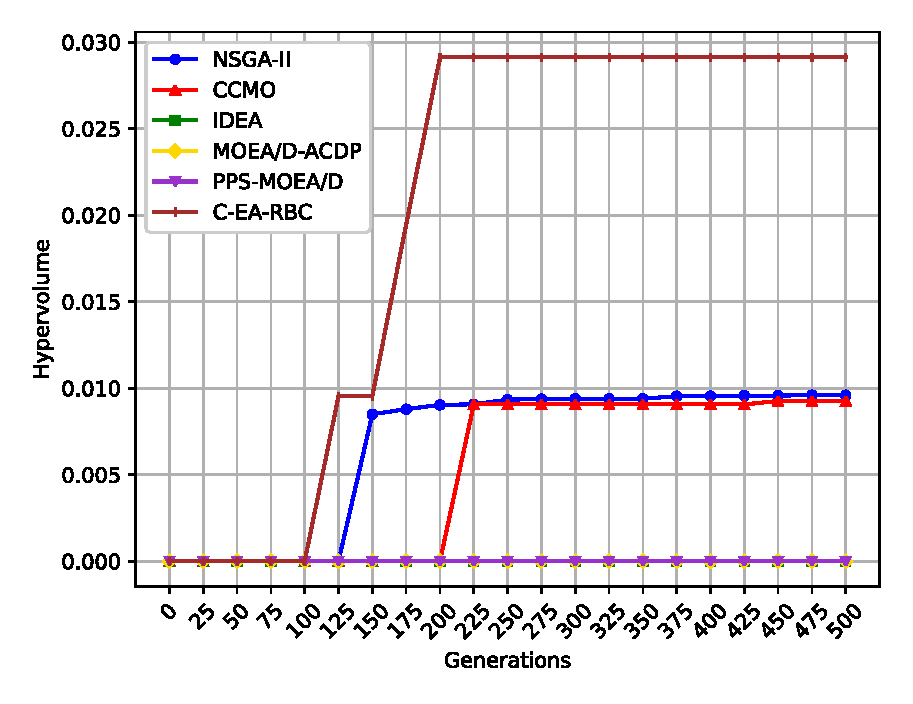
\includegraphics[width=\columnwidth]{figs/HV_gamma400.eps}%
		\vskip-5pt
		\caption{$\gamma=4$}
		\label{fig:HV_gamma400}
	\end{subfigure}\hfill
	\vskip-5pt
	\caption{Average HV when solving SAT-MNK with $M=2$, $K=1$ and varying $\gamma$.}
	\label{fig:HV_CEARBC_gamma}
\end{figure*}	

\section{Experimental Results}

\subsection{Performance Comparison}

We start by analyzing the performance of C-EA-RBC when solving problems with varying levels of constraints. Fig. \ref{fig:HV_CEARBC_gamma} shows the increase in HV over generations for the compared MOEAs when solving SAT-MNK with $N=100$ variables, $M=2$ objectives, $K=1$ epistasis and $\gamma=\{1,2,3,4\}$. In $\gamma=1$ problems, C-EA-RBC, PPS-MOEA/D and IDEA show a slightly better final HV than all other MOEAs, however, a $\gamma$ increases, the performance of IDEA and PPS-MOEA/D decrease significantly, to the point that they do not find any feasible solution in $\gamma \geq 3$ and $\gamma = 4$, respectively. Although NSGA-II, CCMO and MOEA/D-ACDP show lower final HV in $\gamma=1$, they scale better in higher $\gamma$, in particular NSGA-II and CCMO. Nonetheless, C-EA-RBC shows faster HV convergence and higher final HV in $\gamma>1$ problems. 

The difference in the performance of C-EA-RBC in comparison to the compared CMOEAs can be explained by the nature of SAT-MNK, as shown in \ref{fig:sat}. As $\gamma$ increases the PF recedes gradually, meaning that more advanced strategies such as those from PPS-MOEA/D and IDEA cause the search to go past the feasible PF, and gets lost in the infeasible region. On the other hand, the SEA stage of C-EA-RBC searches for feasible solutions without making assumptions on the quality of the solutions, which are then improved by the RBC stage.

\begin{figure}[t!]
	\begin{subfigure}[b]{\columnwidth}
		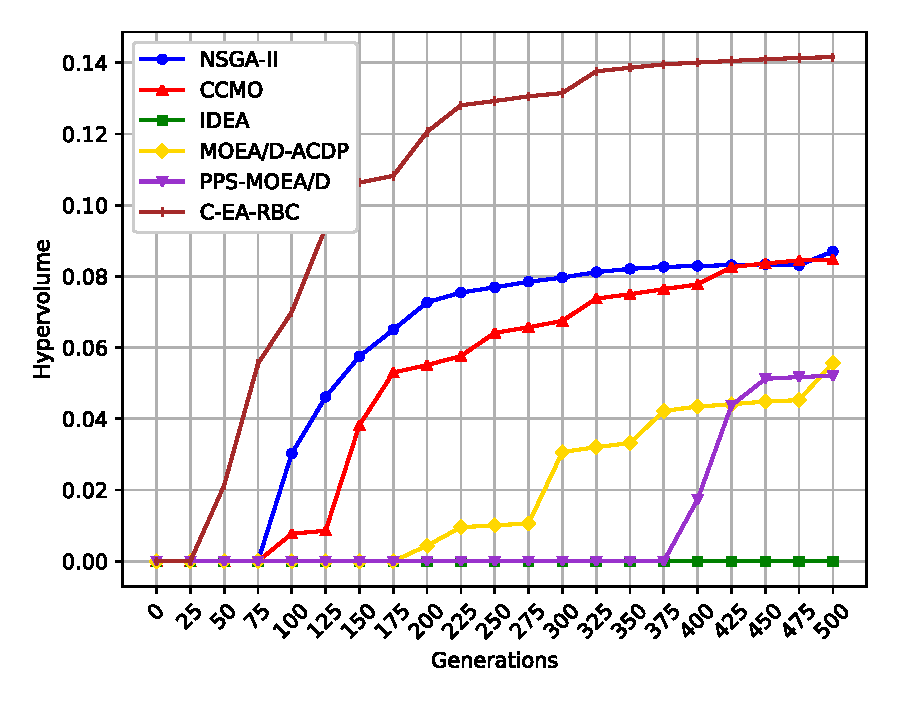
\includegraphics[width=\columnwidth]{figs/HV_nobj3.eps}%
		\vskip-5pt
		\caption{$M=3$.}%
		\label{fig:HV_nobj3}%
	\end{subfigure}\hfill%
	
	\begin{subfigure}[b]{\columnwidth}
		\includegraphics[width=\columnwidth]{figs/HV_nobj4.eps}%
		\vskip-5pt
		\caption{$M=4$.}%
		\label{fig:HV_nobj4}%
		
	\end{subfigure}\hfill%
	\begin{subfigure}[b]{\columnwidth}
		\includegraphics[width=\columnwidth]{figs/HV_nobj5.eps}%
		\vskip-5pt
		\caption{$M=5$.}%
		\label{fig:HV_nobj5}%
	\end{subfigure}\hfill%
	\vskip-5pt
	\caption{HV of C-EA-RBC solving SAT-MNK with $N=100$, $K=1$, $\gamma=3$ and varying $M$.}
	\label{fig:HV_M}
\end{figure}

Next, we analyze how C-EA-RBC scales with larger number of objectives. Fig. \ref{fig:HV_M} shows the average HV value over generations when solving SAT Constrained MNK-Landscapes with $N=100$ variables, $K=1$ epistasis, $\gamma=3$ and $M=\{2,3,4,5\}$ objectives. We can see that C-EA-RBC manages to maintain higher HV values than all the compared MOEAs for all problems solved.


\begin{figure}[t!]
	\begin{subfigure}[b]{\columnwidth}
		\includegraphics[width=\columnwidth]{figs/HV_k3.eps}%
		\vskip-5pt
		\caption{$K=3$.}%
		\label{fig:HV_k3}%
	\end{subfigure}\hfill%
	
	\begin{subfigure}[b]{\columnwidth}
		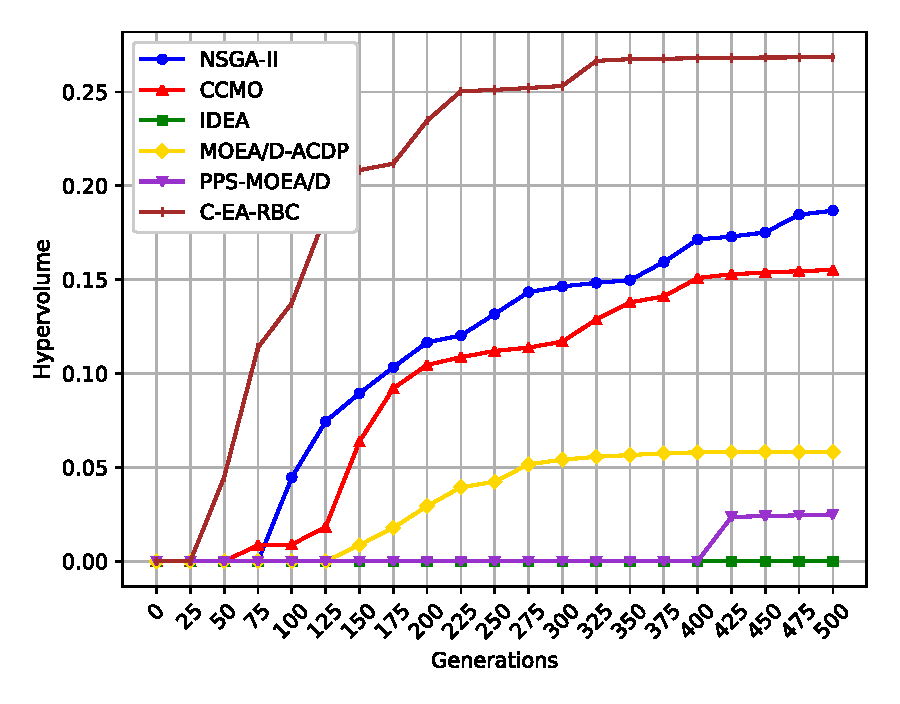
\includegraphics[width=\columnwidth]{figs/HV_k5.eps}%
		\vskip-5pt
		\caption{$K=5$.}%
		\label{fig:HV_k5}%
		
	\end{subfigure}\hfill%
	\begin{subfigure}[b]{\columnwidth}
		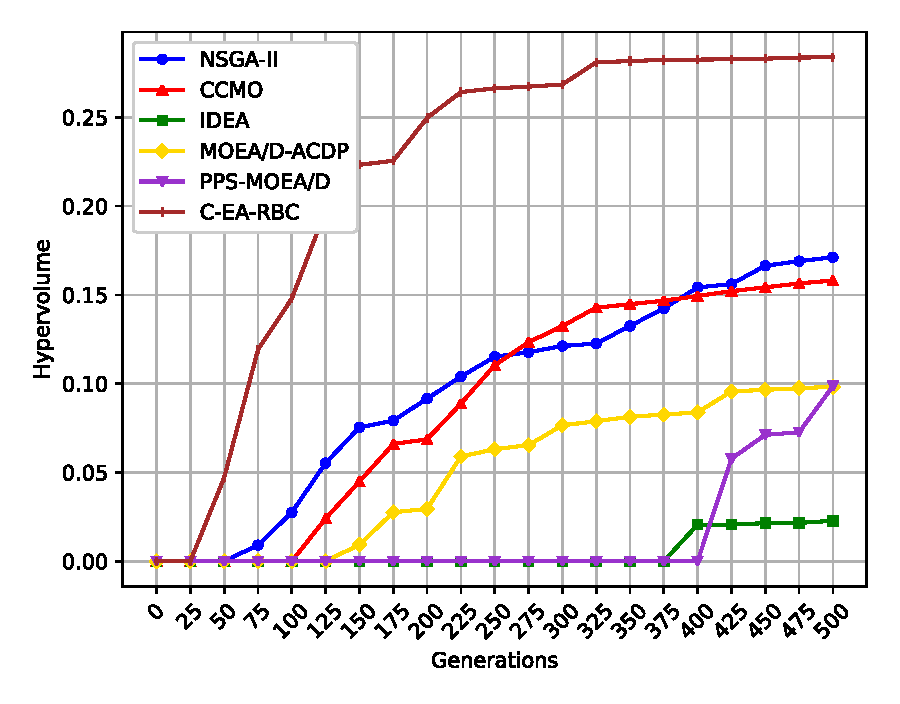
\includegraphics[width=\columnwidth]{figs/HV_k7.eps}%
		\vskip-5pt
		\caption{$K=7$.}%
		\label{fig:HV_k7}%
	\end{subfigure}\hfill%
	\vskip-5pt
	\caption{HV of C-EA-RBC solving SAT-MNK with $M=2$, $N=100$, $\gamma=3$ and varying $K$.}
	\label{fig:HV_k}
\end{figure}

Finally, we study how C-EA-RBC scales with higher level of variable interaction by solving SAT Constrained MNK-Landscapes with $M=2$ objectives, $N=100$ variables, $\gamma=3$ and $K=\{1,3,5,7\}$ epistatic interactions, shown in Fig. \ref{fig:HV_k}. Again, we can see that C-EA-RBC still shows higher HV than all compared HVs for all problem configurations.

%More detail in regards to the performance of C-EA-RBC with different $M$ and $K$ values are given in the following section.

\subsection{Analysis}

\begin{figure}[t!]
	\begin{subfigure}[b]{\columnwidth}
		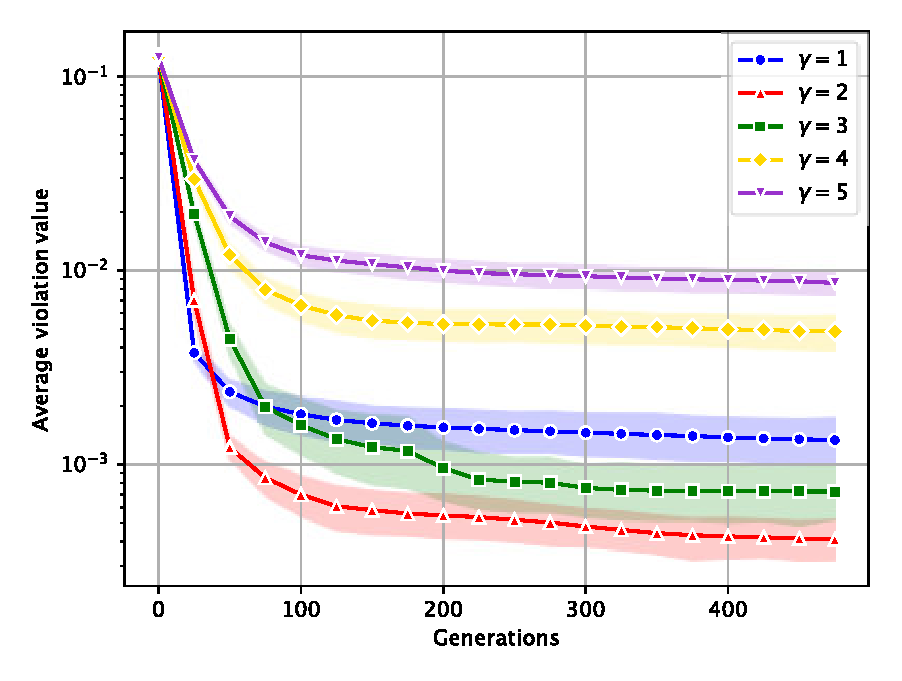
\includegraphics[width=\columnwidth]{figs/vio_gamma.eps}%
		\vskip-5pt
		\caption{$M=2$, $K=1$, $\gamma=\{1,2,3,4,5\}$.}%
		\label{fig:vio_gamma}%
	\end{subfigure}\hfill%
	
	\begin{subfigure}[b]{\columnwidth}
		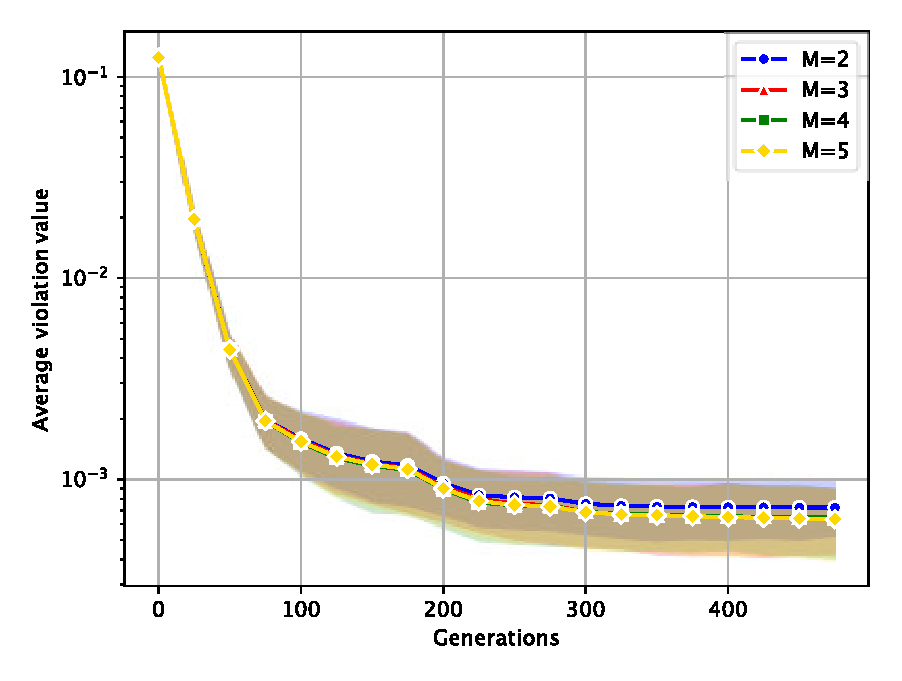
\includegraphics[width=\columnwidth]{figs/vio_M.eps}%
		\vskip-5pt
		\caption{$K=1$, $\gamma=3$, $M=\{2,3,4,5\}$.}%
		\label{fig:vio_M}%
		
	\end{subfigure}\hfill%
	\begin{subfigure}[b]{\columnwidth}
		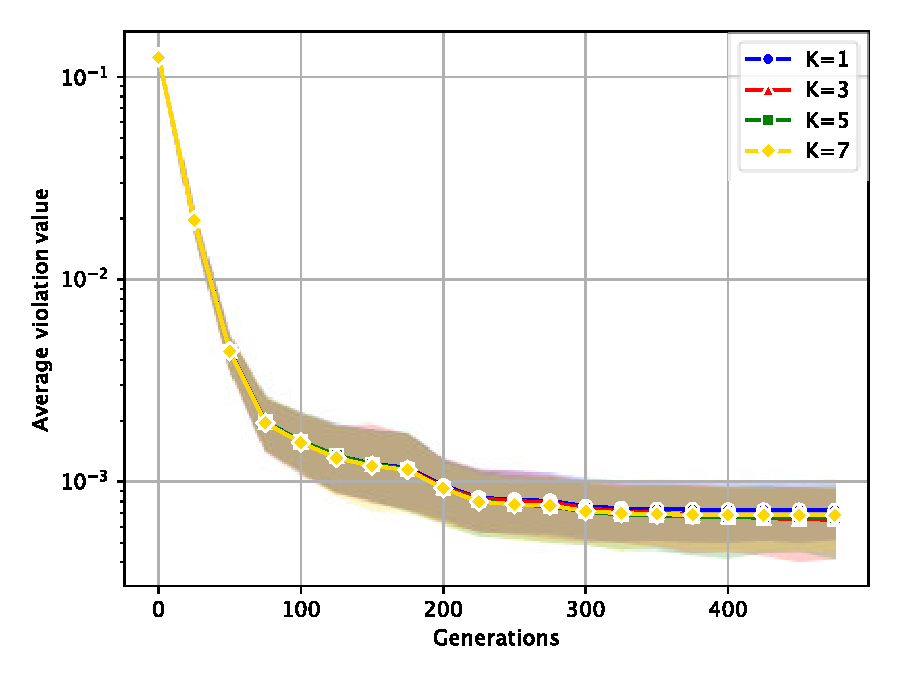
\includegraphics[width=\columnwidth]{figs/vio_K.eps}%
		\vskip-5pt
		\caption{$M=2$, $\gamma=3$, $K=\{1,3,5,7\}$.}%
		\label{fig:vio_K}%
	\end{subfigure}\hfill%
	\vskip-5pt
	\caption{Average violation values of infeasible solutions found by C-EA-RBC solving SAT-MNK with $N=100$ and varying $M$, $K$ and $\gamma$.}
	\label{fig:vio_CEARBC}
\end{figure}

To gain a better insight on how the SEA stage of C-EA-RBC works, we analyze the average constraint violation value of infeasible solutions over generations. Fig. \ref{fig:vio_CEARBC} shows this metric in a logarithmic scale for problems with fixed $M=2$ and $K=1$, varying $\gamma=\{1,2,3,4,5\}$ in Fig. \ref{fig:vio_gamma}, fixed $K=1$ and $\gamma=3$, varying $M=\{2,3,4,5\}$ in Fig. \ref{fig:vio_M}, and fixed $M=2$ and $\gamma=3$, varying $K=\{1,3,5,7\}$ in Fig. \ref{fig:vio_K}. We can see that for $\gamma=1$, C-EA-RBC does not reach very low value of constraint violation. This is likely due to the fact that the constraints in these problems are not very difficult, and the solver can quickly find the first feasible solution and switch to the moRBC stage. In $\gamma=2$ problems, the solver has to spend more time in the SEA stage reducing the constraint violation values until the first feasible solution is found. Then, as $\gamma$ increases, C-EA-RBC has more difficulty reducing the violation value of infeasible solutions. In $\gamma=5$ problems, although it manages to reduce the violation values to a certain extent, is still fails to find any feasible solution before the termination criteria is met. 

When scaling $M$ objectives and $K$ epistatic interactions, as shown in Figs. \ref{fig:vio_M} and \ref{fig:vio_K}, the average constraint violation values are very similar for all problems. Since SEA only optimizes the constraint violations, the number of objectives and epistatic interactions have no impact on its performance, which explains why C-EA-RBC shows better HV than all the other compared CMOEAs in problems with different $M$ and $K$ values.

\begin{figure}[t!]
	\begin{subfigure}[b]{\columnwidth}
		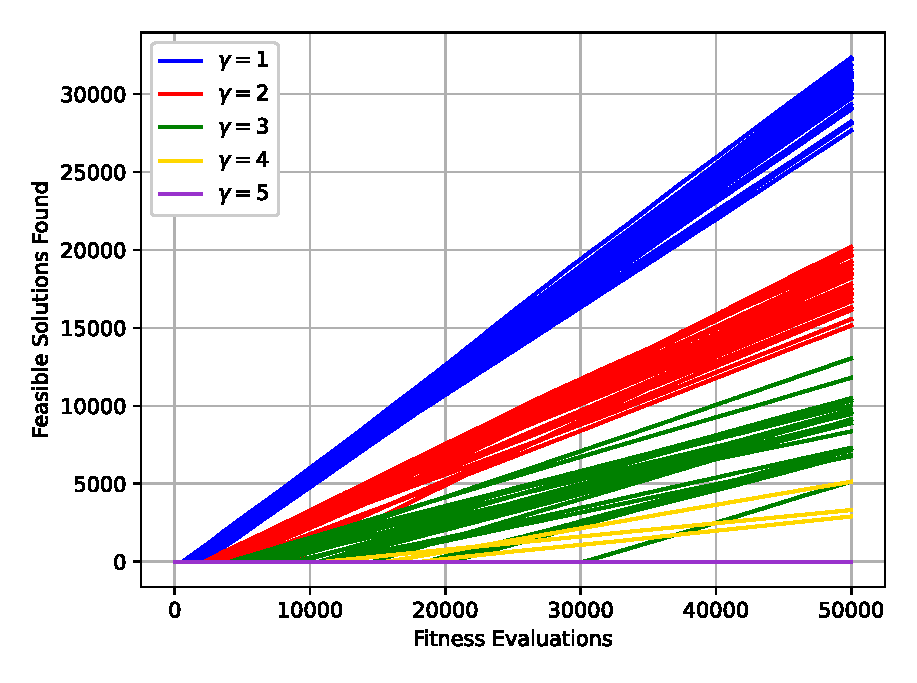
\includegraphics[width=\columnwidth]{figs/ff_gamma.eps}%
		\vskip-5pt
		\caption{$M=2$, $K=1$, $\gamma=\{1,2,3,4,5\}$.}%
		\label{fig:ff_gamma}%
	\end{subfigure}\hfill%
	
	\begin{subfigure}[b]{\columnwidth}
		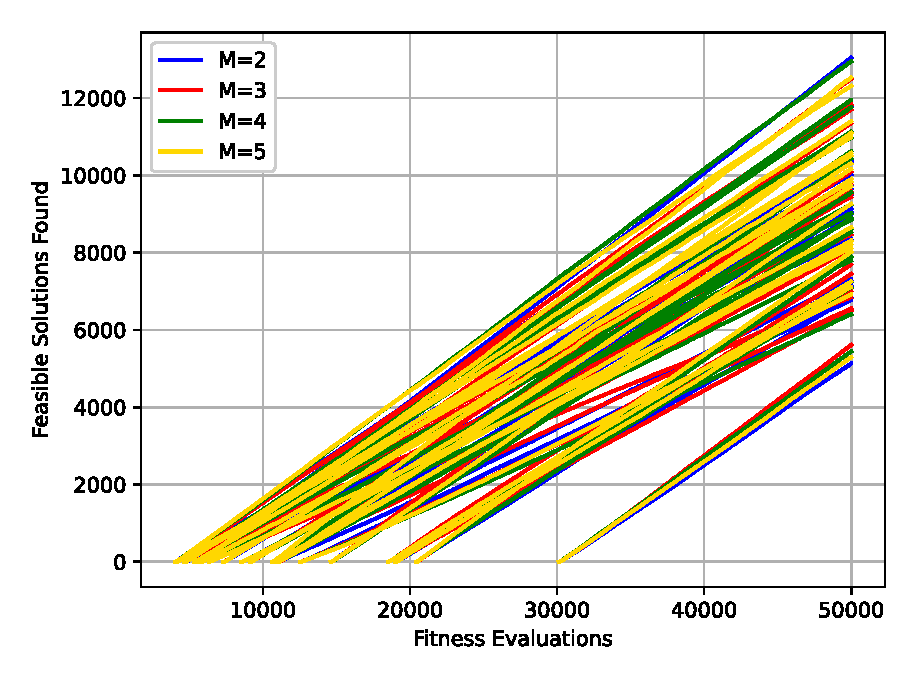
\includegraphics[width=\columnwidth]{figs/ff_M.eps}%
		\vskip-5pt
		\caption{$K=1$, $\gamma=3$, $M=\{2,3,4,5\}$.}%
		\label{fig:ff_M}%
		
	\end{subfigure}\hfill%
	\begin{subfigure}[b]{\columnwidth}
		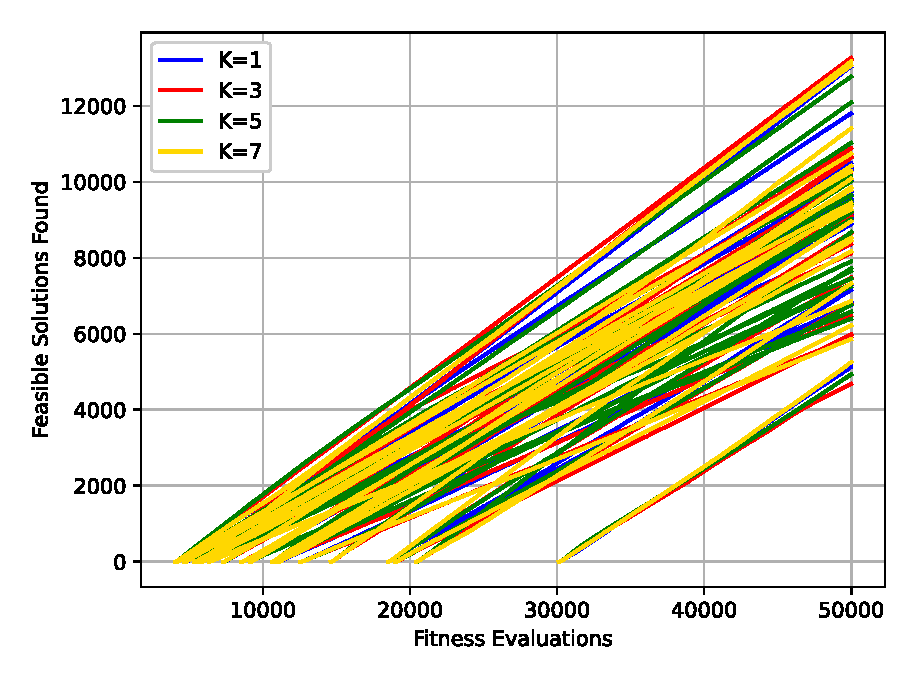
\includegraphics[width=\columnwidth]{figs/ff_K.eps}%
		\vskip-5pt
		\caption{$M=2$, $\gamma=3$, $K=\{1,3,5,7\}$.}%
		\label{fig:ff_K}%
	\end{subfigure}\hfill%
	\vskip-5pt
	\caption{Number of feasible solutions found by C-EA-RBC solving SAT-MNK with $N=100$ and varying $M$, $K$ and $\gamma$.}
	\label{fig:ff_CEARBC}
\end{figure}

Lastly, we analyze the number of feasible solutions found by C-EA-RBC. Figure \ref{fig:ff_CEARBC} shows the number of feasible solutions found in the vertical axis over fitness evaluations in the horizontal axis, where each line represents each SAT Constraint instance solved. For instances where no feasible solution was found, the value is set to 0. Note that this metric does not differentiate if the solution found is non-dominated or not. We can see that moRBC can consistently find additional feasible solutions until the end of the algorithm run, regardless of the problem configuration. In addition, we can see that varying $M$ and $K$ has no significant effect on the efficiency of the moRBC stage of finding feasible solutions, which explains why C-EA-RBC obtains better HV than all the compared CMOEAs in all problem configurations.

\section{Conclusions and Future Works}

In this work, we have presented C-EA-RBC, an MOEA dedicated to solve constrained problems by alternating between a simple EA and an moRBC. The SEA stage aims to find feasible solutions by optimizing constraint violation, while the moRBC stage optimizes the objective functions by climbing non-dominated feasible solutions found by the sEA. We have shown that C-EA-RBC performs well in SAT Constrained MNK-Landscapes with different levels of constraints, number of objectives and number of epistatic interactions. 

In future works, we would like to improve both SEA and morBC stages of C-EA-RBC for a more effective search. Also, we would like to further study C-EA-RBC by solving different CMOPs.

\bibliographystyle{plain}
\bibliography{symposium}

%------------------------------------------------------------------------------
\end{document}
